\documentclass[]{article}

\usepackage{hyperref}
\usepackage{graphicx}
\usepackage{mathtools}
\usepackage{amssymb}
\usepackage[T1]{fontenc}
%\usepackage{enumitem}
\usepackage{paralist}
\usepackage{csquotes}
\usepackage[affil-it]{authblk}
\usepackage{listings}
\usepackage{fixltx2e}
\usepackage[numbers]{natbib}
\usepackage{mathpartir}
\usepackage{mmm}

% Treat paragraph as subsubsubsection
\usepackage{titlesec}
\setcounter{secnumdepth}{4}

\usepackage{tikz}
\usetikzlibrary{shapes,arrows,decorations.pathreplacing,calc}

\DeclareMathOperator{\md5}{MD5}

\lstset{
  frame=none,
  xleftmargin=2pt,
  stepnumber=1,
  numbers=none,
  numbersep=5pt,
  numberstyle=\ttfamily\tiny\color[gray]{0.3},
  belowcaptionskip=\bigskipamount,
  captionpos=b,
  escapeinside={*'}{'*},
  language=haskell,
  tabsize=2,
  emphstyle={\bf},
  commentstyle=\it,
  stringstyle=\mdseries\rmfamily,
  showspaces=false,
  keywordstyle=\bfseries\rmfamily,
  columns=flexible,
  basicstyle=\small\sffamily,
  showstringspaces=false,
  morecomment=[l]\%,
}

\providecommand{\hs}[1]{\lstinline[language=Haskell]|#1|}

\newenvironment{haskell}
  {
    \begin{lstlisting}[language=Haskell, xleftmargin=.2\textwidth, xrightmargin=.2\textwidth]
  }
  {
    \end{lstlisting}
  }

\providecommand{\coq}[1]{\lstinline[language=ML]|#1|}

\begin{document}

\pagestyle{headings}  % switches on printing of running heads

\title{Interestingness Measures for Theory Exploration}

\author{Chris Warburton}

\affil{University of Dundee,\\
\texttt{http://tocai.computing.dundee.ac.uk}}

\maketitle              % typeset the title of the contribution

\begin{abstract}
Since their inception, computers have been applied to automate and assist work in mathematics, with established fields including numerical computation, computer algebra, (online) communication and so on. Here we focus on their use in two areas: formal proof and statistics; and how new approaches are bringing these seemingly disparate disciplines closer together.
\end{abstract}

\section{Introduction}

\iffalse
TODO
Intro + motivation

About 2 pages

Haskell is a mainstream FP language (motivation)

QuickCheck (example)

How to come up with the properties

Mention theory exploration
\fi

As computers and software become more capable, and as our reliance on them increases, the importance of \emph{understanding}, \emph{predicting} and \emph{verifying} these systems grows; which is undermined by their ever-increasing complexity. The \emph{functional programming} paradigm has been proposed for addressing these issues \cite{hughes1989functional}, in part by constructing programs which are more amenable to mathematical analysis. For example, by separating \emph{computation} from \emph{effects}, we can analyse each in isolation; in particular, pure computations can be evaluated without fear of damaging side-effects, and results are repeatable (since there can be no dependence on external state).

Whilst use of pure functional programming languages, like Haskell and Idris, is relatively rare, their features are well suited to common software engineering practices like \emph{unit testing}; where tasks are broken down into small, easily-specified ``units'', and tested in isolation for a variety of use-cases. These ideas are thus spreading to mainstream software engineering, in a more dilute form; seen, for example, in the recent inclusion of first-class functions in Java \cite{gosling2015java} and C++ \cite{willcock2006lambda}.

Although unit testing is the de facto industry standard for quality assurance in non-critical systems, the level of confidence it provides is rather low, and totally inadequate for many (e.g. life-) critical systems. To see why, consider the following Haskell function, along with some unit tests (see \ref{haskell} for more details on Haskell):

\begin{lstlisting}[language=Haskell, xleftmargin=.2\textwidth, xrightmargin=.2\textwidth]
  factorial 0 = 1
  factorial n = n * factorial (n-1)

  fact_base      = factorial 0 == factorial 1
  fact_increases = factorial 4 >  factorial 3
  fact_div       = div (factorial 5) (factorial 4) == 5
\end{lstlisting}

The intent of the function is to map an input $n$ to an output $n!$. The tests check a few properties of the implementation, including the base case, that the function is monotonically increasing, and a relationship between adjacent outputs. However, these tests will \emph{not} expose a serious problem with the implementation: it diverges on half of its possible inputs!

All of Haskell's built-in numeric types allow negative numbers, which this implementation doesn't take into account. Whilst this is a rather trivial example, it highlights a common problem: unit tests are insufficient to expose incorrect assumptions. In this case, our assumption that numbers are positive has caused a bug in the implementation \emph{and} limited the tests we've written.

If we do manage spot this error, we might capture it in a \emph{regression test} and update the definition of \hs{factorial} to handle negative numbers, e.g. by taking their absolute value:

\begin{lstlisting}[language=Haskell, xleftmargin=.2\textwidth, xrightmargin=.2\textwidth]
factorial 0 = 1
factorial n = let nPos = abs n
               in nPos * factorial (nPos - 1)

fact_neg = factorial (-1) == factorial 1
\end{lstlisting}

However, this is \emph{still} not enough: since this function only uses generic numeric operations, it will be polymorphic; allowing all numeric types\footnote{Its type will be of the form \hs{forall t. Num t => t -> t}, where \hs{Num} constrains the type variable \hs{t} to be numeric. There will also be extra contraints like \hs{Eq} due to the use of \hs{==} in the unit tests.}. If we provide a fractional value, the function will again diverge. Clearly, by choosing what to test we are biasing the test suite towards those cases we've already taken into account, whilst neglecting the problems we did not expect.

Haskell offers a partial solution to this problem in the form of \emph{property checking}. Tools such as \textsc{QuickCheck} separate tests into three components: a \emph{property} to check, a source of values to check and a stopping criterion. Here is how we might restate our unit tests as properties:

\begin{lstlisting}[language=Haskell, xleftmargin=.2\textwidth, xrightmargin=.2\textwidth]
fact_base = factorial 0 == factorial 1 -- Unchanged; unit tests are valid (albeit limited) properties

fact_increases n = factorial (n+1) >= factorial n  -- >= since factorial 1 == factorial 0

fact_div n = factorial (n+1) `div` factorial n == n+1

fact_neg n = factorial (n * -1) == factorial n
\end{lstlisting}

Turning particular values (like \hs{5} and \hs{4}) into parameters tells \textsc{QuickCheck} to \emph{universally quantify} them, i.e. a unit test stating $factorial(-1) = factorial(1)$ becomes a property stating $\forall n, factorial(n \times -1) = factorial(n)$.

%TODO example, eg. int -> int -> int requires 2^64 * 2^64 cases for full coverage
%     NO! we want random tests first; show something with edge-cases; what about assuming Ints are positive? what about %assuming Int when it's actually Num

\iffalse

Mathematics provides us with powerful, systematic methods of reasoning, which we can bring to bear on this challenge; in particular those of \emph{formal logic} and \emph{statistics}. By (partially) mechanising these approaches, in the fields of \emph{theorem proving} and \emph{machine learning}, respectively, we can leverage these increasing machine capabilities and direct them for the purpose of analysis. However, the question still remains: on what should we focus that analysis?

In this work, we investigate the notion of \emph{interestingness} in the exploration of formal systems (an area known as \emph{theory exploration}) as a way to make productive use of resources in an often intractable domain. To keep things concrete, we focus our formal analysis on equational formulae describing programs in the Haskell language, for reasons elaborated in \S \ref{haskell}. Conceptually, we maintain a broader view, and survey many related areas which may offer insights on the problem.

Appeals to interestingness arise when more direct measures, such as utility, are not available. For example, the inclusion of particular statements in a program or proof development can be easily justified based on their contribution to the overall solution; however, in a \emph{library} there is no particular problem being solved, in which case we must judge statements on less direct criteria, such as how ``interesting'' they may be to our users. Appeals to interestingness abound in the history of computer-assisted reasoning; for example, in 1971 Plotkin \citep{plotkin1971further} considered the task of \textquote{discovering theorems $T$ from a system of axioms $Ax$}, and in particular the questions \textquote{Under what conditions is $T$ an interesting, possible theorem in the system $Ax$?} and \textquote{Is there a way to generate (most) interesting possible theorems?}. Despite such widespread use of the term, there is no standard definition of what makes a formal object, whether it is an axiom, a conjecture, a proof, etc., ``interesting''; although many ad-hoc heuristics have been proposed.

We begin our undertaking in \S \ref{background} by introducing the Haskell language, as well as the relevant fields of verification for context. We define a formal framework for our investigation, and show how it relates to the existing theorem proving landscape. A selection of theorem proving scenarios which \emph{require} exploration are discussed in \S \ref{examples}, whilst related work, including existing defintions of interestingness, is surveyed in \S \ref{related}. We also review the use of exploration in other fields of Artificial Intelligence and Machine Learning, where researchers are experimenting with replacing \emph{explicit} goals and rewards with \emph{implicit} alternatives such as interestingness. Recent efforts in this area have lead to the emergence of principled theories, mostly based around (algorithmic) information theory, which may be adapted to our theory exploration context.

We discuss our present contributions in \S \ref{current} and future research directions in \S \ref{future}, before concluding in \S \ref{conclusion}.

\fi

\section{Background}
\label{background}

\iffalse
TODO

Background

2.1 Introduce language signature
 a) subset of Haskell DONE
 b) stuff from QuickCheck/Spec

2.2? Machine learning and feature extraction
~1 page

2.3: QuickSpec, HipSpec
\fi

\subsection{Haskell}
\label{haskell}

\newcommand{\fc}{System F\textsubscript{C}}

\begin{figure}
  \begin{equation*}
    \begin{split}
      expr\    \rightarrow\ & \texttt{Var}\ id                                       \\
                         |\ & \texttt{Lit}\ literal                                  \\
                         |\ & \texttt{App}\ expr\ expr                               \\
                         |\ & \texttt{Lam}\ id\ expr                                 \\
                         |\ & \texttt{Let}\ bind\ expr                               \\
                         |\ & \texttt{Case}\ expr\ id\ \left[ alt \right]            \\
      id\      \rightarrow\ & \texttt{Local}\ \mathcal{L}                            \\
                         |\ & \texttt{Global}\ \mathcal{G} \\
      literal\ \rightarrow\ & \texttt{LitNum}\ \mathcal{N}                           \\
                         |\ & \texttt{LitStr}\ \mathcal{S}                           \\
      alt\     \rightarrow\ & ( altcon,\ id,\ expr )                                 \\
      altcon\  \rightarrow\ & \texttt{DataAlt}\ id                                   \\
                         |\ & \texttt{LitAlt}\ literal                               \\
                         |\ & \texttt{Default}                                       \\
      bind\    \rightarrow\ & \texttt{NonRec}\ id\ expr                              \\
                         |\ & \texttt{Rec}\ [ ( id,\ expr ) ]
    \end{split}
  \end{equation*}
  where:
  \begin{tabular}[t]{l @{ $=$ } l}
    $\mathcal{S}$ & string literals    \\
    $\mathcal{N}$ & numeric literals   \\
    $\mathcal{L}$ & local identifiers  \\
    $\mathcal{G}$ & global identifiers
  \end{tabular}

  \caption{Simplified syntax of GHC Core in BNF style. $[]$ and $(,)$ denote repetition and grouping, respectively.}
  \label{coresyntax}
\end{figure}

The full Haskell language is rather complex, so we focus instead on \emph{Core}, an intermediate representation of the Glasgow Haskell Compiler (GHC) based on \fc. For a full treatment of \fc, and its use in GHC, see \citep[Appendix C]{sulzmann2007system}. The sub-set of Core we consider is shown in figure \ref{coresyntax}; compared to the full language \footnote{As of GHC version 7.10.2, the latest at the time of writing.} we erase types and use a custom representation of names. There are also several other forms of literal (machine words of various sizes, individual characters, etc.) which we omit for brevity, as their treatment is similar to those of strings and numerals.

\iffalse

Most work in mechanised, formal mathematics focuses on a \emph{theorem proving} paradigm, usually either \emph{interactive theorem proving} (ITP) or \emph{automated theorem proving} (ATP). Whilst the boundaries between these approaches can be somewhat blurred, we give precise definitions in \S \ref{itp} and \S \ref{atp}, respectively, and characterise both as being \emph{goal-driven}: particular conjectures must be provided as input to the process, and the output is either a proof, a refutation or ``don't know'' (in the case of incomplete procedures).

In this work, we instead adopt the paradigm of \emph{(automated) theory exploration}, discussed in \S \ref{theoryexploration}, which includes the ability to \emph{generate} conjectures, and hence output \emph{novel} theorems. Since many theories will admit an infinite number of trivial theorems (e.g. $\top$, $\top \land \top$, $(\top \land \top) \land \top$, \dots) we require some mechanism for avoiding such undesirable, yet provable, statements. This is the role of interestingness, which we can use to \emph{judge} a statement, in a potentially rich way, rather than merely constructing or failing to construct a proof.

\fi

\subsection{Interactive Theorem Proving}
\label{itp}

ITP is based around a \emph{proof checker} $C$, which is a decision procedure for determining if a given value $P$ (known as a \emph{proof object} or \emph{witness}) consititutes a proof of a given statement $S$:

$$ C \colon (P \times S) \rightarrow Boolean $$

The process of ITP can hence be understood as the search for an appropriate $P$ for our \emph{goal} $S$:

$$ ITP \colon (S \times C) \rightarrow \{ P \mid C(P, S) = True \} $$

It just so happens that a useful way to implement such a system is via pure functional programming, with the result that many ITP systems (AKA \emph{proof assistants}) such as Coq and Agda appear very similar to languages like Haskell. In particular, we can represent statements $S$ as types and proofs $P$ as values, in which case the proof checker $C$ is simply a type-checker. There are some obvious quirks, such as the need to be \emph{total} (not Turing-complete) in order to ensure soundness, but overall many of the features we introduced for Haskell, such as parametricity, type classes and ADTs are directly translatable to the ITP setting.

This coincidence is due to the \emph{Curry-Howard correspondence} \citep{wadler2015propositions}, which identifies programming languages with systems of logic. Functional programming languages correspond to intuitionistic logics, and are hence a natural fit for reasoning on computers. With additional axioms, we can extend these to more familiar classical logics, although these can make it harder to compute.

Most differences between functional programming and ITP stem from different \emph{expectations} of the user. In the case of Haskell, the desire for expressivity outweighs the desire for soundness, and hence its designers opted to make it Turing-complete. For an ITP language like Agda, soundness far outweighs the inconvenience of having to prove termination, so the opposite tradeoff is made. Similarly, since many ITP ``programs'' (proofs) will never be executed, the language can avoid optimisation in favour of simplicity (and hopefully correctness). This approach is summed up by the \emph{de Bruijn criterion}, which requires that the system \textquote{generates 'proof-objects' (of some form) that can be checked by an 'easy' algorithm} \cite[\S~2]{barendregt2001proof}. One nice consequence of this approach, which is followed for example by Isabelle \citep{nipkow2002isabelle} and Coq \citep{bertot2013interactive}, is that the proof assistants themselves can become arbitrarily complex and even buggy, yet as long as the proof checker remains simple we can maintain a high degree of confidence in the results.

Their emphasis on \emph{interactivity}, mostly caused by operating in undecidable domains, means ITP can require an enormous effort for non-trivial proof or verification tasks (e.g. see \citep{hales2015formal}). One common way to mitigate this problem is by implementing powerful \emph{tactics}: meta-programs which automate as much of a proof as possible. The most striking example of such meta-programming is the \emph{Sledgehammer} component of Isabelle/HOL \citep{journals/iandc/MengQP06}, which invokes a multitude of ATP systems on (a translated form of) the current goal to see if any can provide a proof which Isabelle's core checker will accept.

\subsection{Automated Theorem Proving}
\label{atp}

ATP systems are similar in principle to proof assistants, but are based around a \emph{proof search} algorithm rather than a proof checker. By using a fixed algorithm for proving, such as \emph{resolution} \cite[\S~9.6]{Russell:2003:AIM:773294} or \emph{superposition} \citep{bachmair1994rewrite}, ATP programs are limited to particular decidable or semi-decidable fragments of logic. In particular, most ATP systems (such as E \citep{schulz2013system} and Vampire \citep{riazanov2003implementing}) operate in classical first-order logic. This is the most striking difference from ITP systems (e.g. Coq, Agda and Isabelle) which operate in higher-order logics.

In addition to its interest to logicians, ATP has been actively researched in the field of artificial intelligence, dating back to the founding of the field at the 1956 Dartmouth conference. Even by that time Newell and Simon had developed their Logic Theory Machine \citep{newell1956logic}, which was subsequently able to prove theorems like those in Principia Mathematica \citep{newell1958elements}. The approaches now known as \emph{good old-fashioned AI} (GOFAI) were due in part to the success of automated theorem proving, as attempts were made to formulate many problems in a way amenable to these powerful first-order reasoners.

Recently there has been a trend away from this direction, towards statistical formulations amenable to machine learning, which we will review in \S \ref{related}.

\subsection{Theory Exploration}
\label{theoryexploration}

The most striking difference between theory exploration (TE) and theorem proving is the former's lack of an explicit goal (e.g. a user-provided conjecture to prove). Instead, the \emph{implicit} goal is more open-ended: the discovery of ``interesting'' conclusions from the given premises. Of course, a key question to ask is what do we mean by ``interesting''? There is no single answer, although many approximate measures have been proposed. The choice of what counts as interesting has been used to classify various TE implementations \citep{warburtonscaling}, along with their approaches to term generation, well-formedness and proof.

Following \citep{warburtonscaling}, we call a pair $(\Sigma, V)$, of a signature and a set of variables, a \emph{theory}. \emph{Theory exploration} then refers to any process $(\Sigma, V) \overset{TE}{\rightarrow} \text{Terms}(\Sigma, V)$ for producing terms of the theory which are well-formed, provable and ``interesting''.

The conditions of well-formedness and provability can be handled through the use of type systems and automated theorem provers. Hence the method of conjecture generation, and the determination of what is interesting, are the most important properties of any TE system.

Early implementations like \textsc{Theorema} \citep{buchberger2000theory} provided interactive environments, similar to computer algebra systems and interactive theorem provers, to assist the user in finding theorems. Like in the ITP approach, the relatively simple process of verification is automated, whilst the more difficult tasks (term generation and the determination of their interest) are left up to the user.

Subsequent systems have investigated \emph{automated} theory exploration, for tasks such as lemma discovery \citep{Hipster}. By removing user interaction, these properties must be implemented by algorithms. In existing systems these are tightly coupled to improve efficiency, which makes it difficult to try different approaches independently.

As an example, \textsc{QuickSpec} \citep{QuickSpec} discovers equations about Haskell code, which are defined as ``interesting'' if they cannot be simplified using previously discovered equations. The intuition for such criteria is to avoid special cases of known theorems, such as $0 + 0 = 0$, $0 + 1 = 1$, etc. when we already know $0 + x = x$. Whilst this interestingness judgement is elegantly implemented with a congruence closure relation (version 1) and a term rewriting system
(version 2), the conjecture generation is performed in a brute-force way.

Although \textsc{QuickSpec} only \emph{tests} its equations rather than proving them, it is still used as the exploration component of more rigorous systems like \textsc{HipSpec} and \textsc{Hipster}.

\textsc{HipSpec} is currently the most powerful TE system for Haskell, and also forms a major component of \textsc{Hipster}. It uses off-the-shelf ATP programs (including AltErgo, Vampire, Z3, E, SPASS and CVC4) to verify the conjectures of \textsc{QuickSpec}. \textsc{QuickSpec}, in turn, enumerates all type-correct combinations of the terms in the theory up to some depth, groups them into equivalence classes using the \textsc{QuickCheck} counterexample finder, then conjectures equations relating the members of these classes. This approach works well as a lemma generation system, making \textsc{HipSpec} a capable inductive theorem prover as well as a theory exploration system \citep{claessen2013automating}. \textsc{HipSpec} is also compatible with Haskell's existing testing infrastructure, such that an invocation of \texttt{cabal test} can run \textsc{HipSpec} alongside more traditional QA tools like \textsc{QuickCheck}, \textsc{HUnit} and \textsc{Criterion}.

In fact, there are similarities between the way a TE system like \textsc{HipSpec} can generalise from proving \emph{particular} theorems to \emph{inventing} theorems, and the way counterexample finders like \textsc{QuickCheck} can generalise from testing \emph{particular} expressions to \emph{inventing} expressions to test. There are likely lessons that each can learn from the other's approach to term generation.

We identify the following areas for researching potential improvements in existing TE systems such as \textsc{HipSpec}:

\begin{description}
\item{Term generation}:
  Enumerating all type-correct terms is a brute-force solution to this question. Scalable alternatives to brute-force algorithms are a well-studied area of Artificial Intelligence and Machine Learning \iffalse TODO: Related work reference \fi. In particular, heuristic search algorithms like those surveyed in \citep{blum2011hybrid} could be used.
  We could also use Machine Learning methods like those used for \emph{relevance filtering} \ref{relevance} to identify some sub-set of a given theory, to prioritise over the rest.

\item{Interestingness}
  Various alternative interestingness criteria have been proposed, which we survey in \S \ref{relatedwork}. Augmenting or replacing the criteria may be useful, for example to distinguish useful relationships from incidental coincidences; or to prevent surprising, insightful equations from being discarded because they can be simplified.
\end{description}


% Theory exploration is similar to \emph{experimental mathematics}

% - Relation to Science
%  - Testable/falsifiable hypotheses are like evaluable terms (or, more generally, conjectures which can be decided, using a reasonable amount of resources).
% - Relation to AI tasks: exploring surroundings, etc.

% - Statistics is another area that's less straightforward than normal numerical computing, since there is subjectivity and judgement involved in the answering of questions.

% Theory formation: Alison? Others.
% Theory exploration: Buchberger, Moa in Isabelle, Koen in Haskell. Others?
% Theorem proving: Well-trodden: first-order ATP, higher-order ITP, functional programming
% Communication: Latex, Wikis, APIs, communicating with aliens

\section{Exploration in Theorem Proving}
\label{examples}

Before exploring abstract definitions of interestingness, we can first consider some scenarios which arise during formal proof where we are forced to generate conjectures. An analysis of these situations, and the subsequent theorems they produce, will contribute towards an empirical justification for what is interesting (at least from a utilitarian point of view) and inform our later exploration of the literature.

\subsection{Generalisation}

When we \emph{generalise} a statement $S$, we obtain a new statement $S'$ of which $S$ is a special case. Although it seems counterintuitive, a generalised statement can sometimes be \emph{easier} to prove than the original. This arises often in inductive proofs, since the specific obligations which arise in the proof may be incompatible with the available inductive hypotheses.

However, we cannot blindly generalise \emph{all} obligations we encounter, since \emph{over-generalising} results in obligations which are so strong that they are unprovable, or even false. We must therefore rely on heuristics to guide the generation of generalised conjectures, and hence perform a kind of exploration.

An informative example is given by Boyer and Moore of the associativity of multiplication in ACL2 \citep{boyer1983proof}:

$$(x * y) * z = x * (y * z)$$

During the course of the proof, the following obligation arises:

\begin{equation}
  \tag{conc3}
  (y + (x * y)) * z = (y * z) + ((x * y) * z)
  \label{eq:conc3}
\end{equation}

ACL2 automatically generalises \eqref{eq:conc3} by replacing the repeated sub-term $x * y$ with a fresh variable $w$:

\begin{equation}
  \tag{conc4}
  (y + w) * z = (y * z) + (w * z)
  \label{eq:conc4}
\end{equation}

This generalised form is clearly the distributivity law for multiplication and addition, which can be proved separately to the original goal of associativity. It would not be controversial to claim that this distributivity law is interesting in its own right (relative to associativity, at least), in addition to its usefulness in making this proof go through.

% TODO: Describe the ACL2 heuristics

Generalisation also occurs frequently when reasoning about \emph{tail-recursive} definitions \citep{kapur2003automatic}. \footnote{A tail-recursive function can be executed in constant space using a loop, whereas recursion in non-tail positions may require a growing number of stack frames or nested closures. See \S \ref{auxiliarylemmas} for example definitions of each type.}

\subsection{Analogy}

One way to characterise the interestingness of a statement is by \emph{analogy} to existing interesting statements. By finding lemmas analogous to those of a different theory, we may be able to re-use tactics and other forms of meta-programming across both.

Existing theory exploration systems have been successfully applied to this problem, however the use of pure exploration misses opportunities to \emph{focus} the search, since we know which lemmas are used in those theories where a technique succeeded. If we can find an analogy to map from such solved problems to our unsolved goal, we can infer the approximate form of the lemmas we require, and target these specifically.

The approach taken by \textsc{ACL2(ml)} is to find lemmas which may be relevant to solving a goal $G$ by making analogies via unsupervised clustering \citep{Heras.Komendantskaya.Johansson.ea:2013}. These clusters are used in two ways:

\begin{itemize}

  \item First, we use the cluster $C_G$ containing $G$ to identify analogous theorems.

  \item For each theorem $T \in C_G \setminus \{G\}$, we consider those symbols $S_T$ which occur in $T$ but not in $G$. Our analogous lemmas are those used to prove $T$, mutated such that symbols $s \in S_T$ are replaced by members of the cluster $C_s$ containing $s$.

\end{itemize}

The running examples for demonstrating \textsc{ACL2(ml)} are equivalence theorems for tail-recursive and non-tail-recursive calculations, as well as the effect of repeating certain list operations:

\begin{itemize}

  \item $\forall n, \texttt{natp}(n) \rightarrow \texttt{fact-tail}(n) = \texttt{fact}(n)$ where \texttt{natp} is the predicate that $n$ is a natural number, whilst \texttt{fact-tail} and \texttt{fact} are tail-recursive and non-tail-recursive implementations of factorial, respectively.

  \item $\forall n, \texttt{natp}(n) \rightarrow \texttt{power-tail}(n) = \texttt{power}(n)$,  where \texttt{power-tail} and \texttt{power} calculate powers of 2.

  \item $\forall n, \texttt{natp}(n) \rightarrow \texttt{fib-tail}(n) = \texttt{fib}(n)$,  where \texttt{fib-tail} and \texttt{fib} calculate fibonacci numbers.

  \item $\forall x, \texttt{nat-listp}(x) \rightarrow \texttt{sort}(\texttt{sort}(x)) = \texttt{sort}(x)$, for list-of-natural-numbers predicate \texttt{nat-listp} and list-sorting function \texttt{sort}.

  \item $\forall x, \texttt{true-listp}(x) \rightarrow \texttt{rev}(\texttt{rev}(x)) = x$, where \texttt{true-listp} ensures that $x$ is a valid singly-linked list structure and \texttt{rev} is list reversal.

  \item $\forall x, \texttt{true-listp}(x) \rightarrow \texttt{int}(x, x) = x$, where \texttt{int} is the intersection of lists (i.e. a list of elements common to each).

\end{itemize}

\subsection{Auxiliary Lemmas} \label{auxiliarylemmas}

One consideration when generating conjectures is the difference between theorems, lemmas, corollaries, etc. From a logical point of view, these are all equivalent, and hence most proof assistants do not distinguish between them. However, their \emph{intention} may be different: in a sense, theorems are the interesting results; whilst lemmas are useful results, required for proving the theorems.

Some systems, like Coq, allow users to \emph{label} each statement as being a \coq{Theorem}, a \coq{Lemma}, etc. despite their internal representations being the same. This shows us immediately that lemmas outnumber theorems; in the Coq standard library there are over five times as many lemmas as theorems \footnote{The latest version as of writing is \texttt{coq-8.4pl6} which, when excluding comments, includes 1492 occurences of \coq{Theorem} and 7594 of \coq{Lemma} in its \texttt{theories/} directory.}.

% TODO: Analyse them

% TODO: Theory exploration as lemma generation; give example from a HipSpec paper

We can find a need for auxiliary lemmas, once again, in the context of tail-recursive functions. Consider proving the (pointwise) equality of the following Coq functions, defined for the Peano naturals \coq{Z} and \coq{S}:

\begin{lstlisting}[language=ML, xleftmargin=.2\textwidth, xrightmargin=.2\textwidth]
Inductive Nat : Set := Z : Nat
                     | S : Nat -> Nat.

Fixpoint plus      (n m : Nat) := match n with
                                      | Z    => m
                                      | S n' => S (plus n' m)
                                  end.

Fixpoint plus_tail (n m : Nat) := match n with
                                      | Z    => m
                                      | S n' => plus_tail n' (S m)
                                  end.
\end{lstlisting}

\iffalse

Haskell equivalent:

plus :: Nat -> Nat -> Nat
plus      n  Z    = n
plus      n (S m) = S (plus n m)

plus_tail :: Nat -> Nat -> Nat
plus_tail n  Z    = n
plus_tail n (S m) = plus_tail (S n) m

\fi

Both of these functions implement addition, but the \coq{plus_tail} variant is tail-recursive. However, if we want to \emph{prove} that the definitions are (pointwise) equal, we run into difficulties. In particular, when the inductive step requires us to prove \coq{plus (S n) m = plus n (S m)} (which seems reasonable), we cannot make this go through using another inductive argument.

\iffalse

\begin{lstlisting}[language=ML, xleftmargin=.2\textwidth, xrightmargin=.2\textwidth]
(* Solve equalities by beta-normalising both sides *)
Ltac triv := try (simpl; reflexivity).

(* Prove equivalence of plus and plus_tail *)
Theorem equiv : forall n m, plus n m = plus_tail n m.
  induction n; triv. (* Base case is trivial *)

  (* Inductive case: plus (S n) m = plus_tail (S n) m *)
  intro m.

  (* Beta-reduce the right-hand-side (justification is trivial) *)
  replace (plus_tail (S n) m) with (plus_tail n (S m)); triv.

  (* Use induction hypothesis to replace plus_tail with plus *)
  rewrite <- (IHn (S m)).
\end{lstlisting}

\fi

Specifically, the \emph{conclusion} of a second inductive hypothesis is exactly the equation we need:

\begin{lstlisting}[language=ML, xleftmargin=.2\textwidth, xrightmargin=.2\textwidth]
IHn' : (forall x, plus n' x = plus_tail n' x) -> plus (S n') m = plus n' (S m)
\end{lstlisting}

Yet we cannot provide it with the argument it needs, as our original induction hypothesis is \emph{too specific} (i.e. it has too many \coq{S} constructors):

\begin{lstlisting}[language=ML, xleftmargin=.2\textwidth, xrightmargin=.2\textwidth]
IHn : forall x, plus (S n') x = plus_tail (S n') x
\end{lstlisting}

We are forced to abandon the proof, despite such a reasonable-looking intermediate goal.

In fact, if we attempt to prove that goal \emph{separately}, we can use a straightforward argument by induction; even though it is actually \emph{stronger} due to the absence of the \coq{IHn} assumption. Using this separate result as a lemma, the pointwise equality is proven easily.

\iffalse

\begin{lstlisting}[language=ML, xleftmargin=.2\textwidth, xrightmargin=.2\textwidth]
Lemma gen n m : plus (S n) m = plus n (S m).
  induction n; triv. (* Base case is trivial *)

  (* Move all S constructors outside *)
  simpl. rewrite <- IHn. simpl.

  (* Trivial *)
  reflexivity.
Defined.
\end{lstlisting}

\begin{lstlisting}[language=ML, xleftmargin=.2\textwidth, xrightmargin=.2\textwidth]
  rewrite (gen n m).
  reflexivity.
Defined.
\end{lstlisting}

\fi

\subsection{Tests} \label{tests}

Since we are working in the domain of Haskell programs, an abundant source of statements are available in the form of \emph{tests}. For manually-written tests, the effort required to write them implies that they must be of some interest to their author. Many forms of test are \emph{not} suitable for our purposes, such as \emph{unit tests} which are always trivially provable by $\beta$-reduction; or \emph{integration tests}, which depend on the behaviour of the external environment. One reason to study Haskell is its widespread use of \emph{property checking}, which does give us useful data. Many Haskell property checkers exist, based on random testing (\textsc{QuickCheck} \citep{claessen2011quickcheck} and \textsc{SmartCheck} \citep{pike2014smartcheck}), enumeration (\textsc{SmallCheck} \citep{runciman2008smallcheck}), observation (\textsc{Lazy SmallCheck} \citep{reich2013advances}) and logic programming (\textsc{SparseCheck} \citep{sparsecheck}).

Thankfully the major differences between these systems are in the way they instantiate test arguments; their representations of properties are largely the same (modulo renaming of functions and types).

Here we consider the 10 most-downloaded packages from \textsc{Hackage} (as of 2015-10-30) which have property tests; these are \texttt{warp}, \texttt{aeson}, \texttt{text}, \texttt{lens}, \texttt{conduit}, \texttt{pandoc}, \texttt{attoparsec}, \texttt{scientific}, \texttt{yesod-core} and \texttt{blaze-html}.

% TODO: Analysis

\section{Contributions}\label{current}

\iffalse
TODO

3 Recurrent clustering

Good analysis of differences with ML4PG/ACL2ML
\fi

\section{Implementation}

Most of the work carried out so far has been either preliminary investigations, to determine if a particular approach is worth pursuing; or at an infrastructure level to support experimentation.

\subsection{Circular Convolution}\label{circularconvolution}

We have investigated the reduction to a fixed-size of tree structures of the following form (where \hs{FV} denotes a feature vector):

\begin{lstlisting}[language=Haskell, xleftmargin=.2\textwidth, xrightmargin=.2\textwidth]
data Tree = Leaf FV
          | Branch FV Tree Tree
\end{lstlisting}

Just like in the non-recursive case, the simplest way to reduce our dimensionality is to truncate. To reduce an arbitrary \hs{t :: Tree} to a maximum depth \hs{d > 0}, we can use \hs{reduceD d t} where:

\begin{lstlisting}[language=Haskell, xleftmargin=.2\textwidth, xrightmargin=.2\textwidth]
reduceD 1 (Branch fv l r) = Leaf   fv
reduceD n (Leaf   fv)     = Leaf   fv
reduceD n (Branch fv l r) = Branch fv (reduceD (n-1) l)
                                      (reduceD (n-1) r)
\end{lstlisting}

This is simple, but suffers two problems:

\begin{itemize}
 \item We must choose a conservatively large \hs{d}, since we're throwing away information
 \item The number of feature vectors grows exponentially as \hs{d} increases
\end{itemize}

The first problem can't be avoided when truncating, but the second can be mitigated by truncating the \emph{width} of the tree as well, to some \hs{w > 0}. One way to truncate the width is tabulating the tree's feature vectors, then truncating the table to \hs{w} $\times$ \hs{d}, as ML4PG does.

\iffalse

We can do this with \hs{tabulate w d t}:

\begin{lstlisting}[language=Haskell, xleftmargin=.2\textwidth, xrightmargin=.2\textwidth]
tabulate w d t = take d (map (take w) (tabulate' t))

tabulate' (Leaf   fv)     = [fv] : []
tabulate' (Branch fv l r) = [fv] : merge (tabulate' l) (tabulate' r)

merge    []     ys  = ys
merge    xs     []  = xs
merge (x:xs) (y:ys) = (x ++ y) : merge xs ys
\end{lstlisting}

\fi

Rather than truncating our trees, we can \emph{combine} the feature vectors of leaves into their parents, and hence \emph{fold} the tree up to any finite depth. Following \citep{zanzotto2012distributed} we have investigated the use of \emph{circular convolution} (\hs{cc}) as our combining function. Hence, to reduce \hs{t :: Tree} to a single feature vector, we can use \hs{reduceC t} where:

\begin{lstlisting}[language=Haskell, xleftmargin=.2\textwidth, xrightmargin=.2\textwidth]
reduceC (Leaf fv)       = fv
reduceC (Branch fv l r) = cc fv (cc (reduceC l) (reduceC r))
\end{lstlisting}

Circular convolution has the following desirable properties:

\begin{description}

  \item{Non-commutative}: \hs{cc a b} $\not\approx$ \hs{cc b a}, hence we can distinguish between \hs{Branch fv a b} and \hs{Branch fv b a}

  \item{Non-associative}: \hs{cc a (cc b c)} $\not\approx$ \hs{cc (cc a b) c}, hence we can distinguish between \hs{Branch v1 a (Branch v2 b c)} and \hs{Branch v1 (Branch v2 a b) c)}.

\end{description}

Here we use $\not\approx$ to represent that these quantities differ \emph{with high probability}, based on empirical testing. This is the best we can do, since the type of combining functions \hs{(FV, FV) -> FV} has a co-domain strictly smaller than its domain, and hence it must discard some information. In the case of circular convolution, the remaining information is spread out among the bits in the resulting feature, which is known as a \emph{distributed representation} \citep{conf/ijcai/Plate91}.

Distributed representations mix information from all parts of a structure together into a fixed number of bits, storing an \emph{approximation} whose accuracy depends on the size of the value and the amount of storage used.

\subsubsection{Extracting Features from XML}

This method of folding with circular convolution has been implemented in the Haskell program \textsc{Tree Features} \footnote{Available online at \href{http://chriswarbo.net/git/tree-features}{http://chriswarbo.net/tree-features}. The application parses arbitrary trees of XML and uses binary features, ie. feature vectors are bit vectors.

To calculate the initial feature of an XML element, before any folding occurs, we concatenate its name and attributes to produce a string \hss}. The feature is then:

\begin{equation}
feature(n) = 2^{\md5(s) \pmod{L}}
\end{equation}

Where $\md5$ is the MD5 hash algorithm and $L$ is the length of the desired vector, given as a commandline argument. The result of $feature(s)$ is a bit vector of length $L$, containing only a single $1$. Due to the use of a hashing function, the position of that $1$ can be deterministically calculated from the input $s$, yet the \emph{a priori} probability of each position is effectively uniform.

In other words, the hash introduces unwanted patterns which are \emph{theoretically} learnable, but in practice a strong hash can be treated as irreversible and hence unlearnable.

\subsubsection{Application to Coq}

Prior to 2014-09-08, the Coq proof assistant provided a rudimentary XML import/export feature, which we can use to access tree structures for learning. We achieve this by using the \coq{external} primitive of the Ltac tactic language: \coq{external "treefeatures" "32" t1 t2 t3.} will generate an XML tree representing the Coq terms \coq{t1}, \coq{t2} and \coq{t3}, and send it to the standard input of a \texttt{treefeatures} invocation, using a vector length argument of 32.

Coq will also interpret the standard output of the command, to generate terms and tactics. This functionality isn't yet used by \textsc{Tree Features}, but it is clear that a feedback loop can be constructed, allowing the construction of powerful \textsc{Ltac} tactics which invoke external machine learning systems.

\subsection{\texttt{nix-eval}}\label{nixeval}

To facilitate theorem proving and machine learning, our theory exploration experiments require access to the \emph{definitions} of the terms under investigation. This is difficult, as many terms are functions, which Haskell does not let us inspect. This limitation can be worked around by programming at a meta-level: manipulating \emph{representations} of Haskell expressions, rather than the expressions themselves. To retain our ability to \emph{evaluate} expressions, we then need a mechanism to transform these representations into the expressions they represent; this usually takes the form of an \texttt{eval} function.

\texttt{eval} is a common feature in languages such as Python and Javascript, where extra source files can be imported dynamically. In that case \texttt{eval} can be implemented easily by representing expressions as strings, then treating those strings as if they were the content of a file being imported.

On the other hand, Haskell does not natively support dynamic importing of extra source files, making implementation of \texttt{eval} trickier. Comprehensive implementations do exist, such as \texttt{hint}, which are effectively wrappers around GHC, but all are limited to using the Haskell modules which are already installed on the system. Since we want to explore \emph{arbitrary} Haskell code, this is not enough for our purposes.

We have implemented a library called \texttt{nix-eval}, which provides an \hs{eval} function for Haskell expressions which may reference packages that are not installed on the system. These packages will be automatically downloaded and installed into a sandbox when a call to \hs{eval} is forced.

\texttt{nix-eval} is build on top of the Nix package manager and GHC. Nix provides a language for defining packages, a \texttt{cabal2nix} tool for generating Nix package definitions from those of Haskell's Cabal tool, and a \texttt{nix-shell} tool for evaluating arbitrary shell commands in a sandbox containing arbitrary packages.

The internal representation of \texttt{nix-eval} includes a list of package names, a list of module names, a list of GHC options and a string containing Haskell code. When evaluated, \texttt{nix-shell} is invoked to create a sandbox containing an instance of GHC and the Haskell packages listed in the expression. GHC is invoked in this sandbox using the \texttt{runhaskell} command, along with any options given in the expression. The code to be evaluated is prepended with \hs{import} statements for each required module, and wrapped in a simple \hs{main} function for printing the result of its evaluation to standard output. The expression, therefore, must have type \hs{String}; although this is not enforced statically.

The type of the \hs{eval} function is \hs{Expr -> IO (Maybe String)}, where \hs{Expr} is the type of expressions described above. The \hs{IO} wrapper comes from our invocation of external tools, and \hs{Maybe String} allows us to represent failure in a clean way. The restriction of expressions to \hs{String}s is not onerous; some concrete type is required, to communicate results from the GHC invocation, but we consider the particular choice of encoding to be out of scope for \texttt{nix-eval}. It would be a straightforward exercise to wrap our \hs{eval} function in a generic encoding mechanism, e.g. using JSON.

\subsection{\textsc{ASTPlugin}}\label{astplugin}

The Glasgow Haskell Compiler provides mechanisms for parsing Haskell code into tree structures, and a \emph{renaming} transformation which makes all names unique; either by prefixing them with the name of the module which defines them, or by suffixing the name with a number. This allows us to spot repeated use of a term, across multiple modules and packages, with a simple syntactic equality check.

Since we are interested in comparing definitions based on the terms they reference, building our framework on top of GHC seems like a promising approach. Indeed, \textsc{HipSpec} already invokes GHC's API to obtain the definitions of Haskell functions, in order to transform them into a form suitable for ATP systems. However, our initial experiments showed that this technique is too fragile for use on many real Haskell projects.

This is due to many projects having a complex module structure, requiring particular GHC flags to be given, or using pre-processors such as \texttt{cpp} and Template Haskell to generate parts of their code. All of this complexity means that invoking GHC ``manually'' via its API is unlikely to obtain the definitions we require.

Thankfully there is one implementation detail which most Haskell packages agree on: the Cabal build system. All of the above complexities can be specified in a package's ``Cabal file'', such that the \texttt{cabal configure} and \texttt{cabal build} commands are very likely to work for most packages, without any extra effort. This shifted our focus to augmenting GHC and Cabal, such that definitions can be collected during the normal Haskell build process.

GHC provides a plugin mechanism for manipulating its Core representation, intended for optimisation passes, which we use to inspect definitions as they are being compiled. We provide a plugin called \textsc{AstPlugin} which implements an optimisation pass which returns its argument unchanged, but which also emits a serialised version of the definition to the console.

There are several complications in the implementation of \textsc{AstPlugin}. We are working with Core, which as a variant of System F\textsubscript{C} \citep{sulzmann2007system} has slightly different syntax and semantics to Haskell. This is mostly a benefit, since Core is a much simpler language than Haskell and its representation is relatively stable compared to many existing representations of Haskell (which often change to support various language extensions). Three areas which make Core more difficult to handle are:

\begin{description}
  \item{Type variables}: In \S \ref{haskell} we saw that parametric polymorphism can be thought of as values being parameterised by type-level objects. In System F, this is represented explicitly by a special binding form $\Lambda$, distinct from the $\lambda$ binding form for value parameters. Core also has explicit bindings for type-level objects, although for simplicity it uses the same $\lambda$ representation for both types and values. This difference from Haskell, which only has explicit binding of values, alters function properties like arity.

  \item{Unified namespace}: Haskell has distinct namespaces for values, types, data constructors, etc. Since Core does not make these distinctions, names may become ambiguous. For example, a type parameter \hs{t} may be confused with a function argument \hs{t}. To prevent this, overlapping namespaces are distinguished by prefices which are distinct from the available names; for example a type class constraint \hs{Ord t} may give rise to a binder \texttt{$\lambda$ \$dOrd} in Core. This causes difficulties when looking up names, as these prefixed forms do not easily map back to the Haskell source.

  \item{Violating encapsulation}: As discussed in \S \ref{haskell}, Haskell allows names to be \emph{private} to a module. When compiling Core, we have full access to private definitions, as well as references to private names from within other definitions. Hence the definitions we receive from \textsc{AstPlugin} will include private values which we cannot import into a theory exploration tool.
\end{description}

In practice, we work around these issues with a post-processing stage: for each named definition appearing in the output of \textsc{AstPlugin}, we attempt to type-check a Haskell expression which imports that name and passes it to \textsc{QuickSpec}. Those which fail, due to the reasons above and others, are discarded.

The result of building a Haskell package with \textsc{AstPlugin} is a database of Haskell definitions, similar in some respects to \textsc{Hoogle}. Definitions are indexed by a combination of their package name, module name and binding name. The definitions themselves are s-expressions representing the Core AST, with non-local references replaced by a combination of package name, module name and binding name (AKA database keys). Each definition also has an associated arity and type, obtained during the post-processing step mentioned above.

Such data is useful for multiple purposes:

\begin{itemize}
  \item{Dependency tracking}: We have a tool which annotates each definition with its dependencies, i.e. those (package, module, name) combinations which it references. Definitions are then topologically sorted into dependency order, as this is required for our recurrent clustering technique.

  \item{Machine learning}: The Core s-expressions are used as input to our machine learning approaches, for guiding theory exploration using statistical properties of the theory being explored. As mentioned in \S \ref{featureextraction}, it is inefficient to apply intensive machine learning algorithms directly to high-dimensional data representations, so we use various feature extraction algorithms to reduce their dimensionality.

  \item{Theory exploration}: The \textsc{MLSpec} tool, described below, uses the output of \textsc{AstPlugin} to construct theories suitable for \textsc{QuickSpec} to explore.

  \item{Reflection}: As mentioned above, \textsc{HipSpec} uses the GHC API to obtain definitions of Haskell terms, which are then converted for use by theorem provers. Although we have not yet investigated this use, it seems likely that the output of \textsc{AstPlugin} would provide a more comprehensive and robust alternative to the GHC API approach.

  \item{Counterexample Generation}: As mentioned in \S \ref{tests}, there are many Haskell property checkers, which differ mostly in the way they generate values for testing. Since our theory exploration tools are built on these property checkers, we rely on the existence of value generators for at least some of the types in our theory; yet existing approaches to deriving such generators (e.g. as found in the \texttt{derive} package) rely on choosing an arbitrary constructor then recursing. As demonstrated in \S \ref{haskell}, a type's constructors might not be exported, in which case these methods fail. Also, the exponential complexity of such naive recursion makes these generators unusable in many cases. It seems that a database of inspectable Haskell functions may be useful for solving this problem in a more practical way, although we have not yet performed experiments in this area.
\end{itemize}

\subsection{\textsc{MLSpec}}\label{mlspec}

When investigating heuristic methods like those of machine learning, it is important to use as much realistic data as possible to predict the system's performance on real tasks. One bottleneck for theory exploration is the lack of theories which are available to explore: we must manually select a set of terms to explore, and sometimes specify variables too.

Our \textsc{MLSpec} tool can automatically build theories suitable for exploration by \textsc{QuickSpec}, based on the databases constructed by \textsc{AstPlugin} described above. Features of \textsc{MLSpec} include:

\begin{itemize}
  \item{Monomorphising}: Given values of polymorphic type, e.g. \hs{safeHead :: forall t. [t] -> Maybe t} and \hs{[] :: forall t. [t]}, a testing-based system like \textsc{QuickSpec} is unable to evaluate expressions such as \hs{safeHead [] :: forall t. Maybe t} without instantiating the variable \hs{t} to a specific type. Such an instantiation is called \emph{monomorphising}, and in the case of \textsc{MLSpec} we build on previous work in \textsc{QuickCheck} by attempting to instantiate all type variables to \hs{Integer}. We discard those cases where this is invalid, such as variable \emph{type constructors} (e.g. \hs{forall c. c Bool -> c Bool}) or incompatible class constraints (e.g. \hs{forall t. IsString t => t}).

  \item{Qualification}: All names are \emph{qualified} (prefixed by their module's name), to avoid most ambiguity. There is still the possibility that multiple packages will declare modules of the same name, in which case the exploration process will abort.

  \item{Variable definition}: Once a \textsc{QuickSpec} theory has been defined containing all of the given terms, we inspect the types it references and append three variables for each to the theory (enough to discover laws such as associativity, but not too many to overflow the limit of \textsc{QuickSpec}'s exhaustive search).

  \item{Sandboxing}: \textsc{MLSpec} is built on top of \texttt{nix-eval}, which allows the theory being explored to reference packages which aren't yet installed on the system.

\end{itemize}

\subsection{\textsc{ML4HS}}\label{ml4hs}

\textsc{ML4HS} is our top-level theory exploration framework, combining \textsc{AstPlugin}, \textsc{TreeFeatures}, the \textsc{Weka} machine learning library and \textsc{MLSpec}.

Inspired by the use of premise selection (see \S \ref{relevance}) to reduce the search space in ATP,
we select sub-sets of the given theory to explore, chosen to try and keep together those expressions which combine in interesting ways, and to separate those which combine in uninteresting ways.

We hypothesise that similarity-based clustering of expressions, inspired by those of \textsc{ML4PG}  and related work in \textsc{ACL2(ml)} (see \S \ref{clustering}), is an effective method for performing this separation.

% TODO: Future experiments will test this by comparing the throughput of \textsc{QuickSpec} with and without the \textsc{ML4HS} pre-processor.

% Divide and conquer for theory exploration
% Does it help?

% Clustering and feature extraction

\section{First Results}

\iffalse
TODO

Future work?
Hypothetical use cases?
\fi

\section{Related Work}
\label{related}

\subsection{Haskell}
\label{haskelldesc}

Firstly, however, we give an overview of the Haskell programming language in \S \ref{haskell}. This allows us to establish many concepts in a straightforward software context, which we can then re-use in the potentially less-familiar realm of interactive theorem proving. We decided to focus on Haskell as it has mature, state-of-the-art theory exploration implementations (\textsc{QuickSpec} \citep{QuickSpec} and \textsc{HipSpec} \citep{claessen2013automating}). This is evident from the fact that the state-of-the-art equivalent for Isabelle/HOL, the \textsc{Hipster} \citep{Hipster} system, is actually implemented by translating to Haskell and invoking \textsc{HipSpec}.

Haskell is a programming language which is well-suited to research; indeed, this was a goal of the language's creators \citep{marlow2010haskell}. Like most members of the \emph{functional programming} paradigm, Haskell is essentially a variant of $\lambda$-calculus; in fact the \textsc{GHC} compiler uses (variants of) the polymorphic $\lambda$-calculus \emph{System F} as an intermediate representation (referred to as \emph{GHC Core}). For a detailed exposition of the language syntax and semantics, you can consult the Haskell Language Report \citep{marlow2010haskell} \footnote{Version 2010 was current as this was written} or a textbook such as \citep{thompson1999haskell}; here we will focus on those language features which make it particularly suited for our formal reasoning purposes:

\begin{description}

\item{Functional}: All control flow is performed by function abstraction and application, which we can reason about using standard rules of inference such as \emph{modus ponens}.

\item{Pure}: Execution of actions (e.g. reading files) is separate to evaluation of expressions; hence our reasoning can safely ignore complicated external and non-local interactions.

\item{Statically Typed}: Expression are constrained by \emph{types}, which can be used to eliminate unwanted combinations of values, and hence reduce search spaces; \emph{static} types can be deduced syntactically, without having to execute the code.

\item{Non-strict}: If an evaluation strategy exists for $\beta$-normalising an expression (i.e. performing function calls) without diverging, then a non-strict evaluation strategy will not diverge when evaluating that expression. This is rather technical, but in simple terms it allows us to reason effectively about a Turing-complete language, where evaluation may not terminate. For example, when reasoning about \emph{pairs} of values \hs{(x, y)} and projection functions \hs{fst} and \hs{snd}, we might want to use an ``obvious'' rule such as $\forall \text{\hs{x y}}, \text{\hs{x}} = \text{\hs{fst (x, y)}}$. Haskell's non-strict semantics makes this equation valid; whilst it would \emph{not} be valid in the strict setting common to most other languages, where the expression \hs{fst (x, y)} will diverge if \hs{y} diverges (and hence alter the semantics, if \hs{x} doesn't diverge).

\item{Algebraic Data Types}: These provide a rich grammar for building up user-defined data representations, and an inverse mechanism to inspect these data by \emph{pattern-matching}. For our purposes, the useful consequences of ADTs and pattern-matching include their amenability for inductive proofs and the fact they are \emph{closed}; i.e. an ADT's declaration specifies all of the normal forms for that type. This makes exhaustive case analysis trivial, which would be impossible for \emph{open} types (for example, consider classes in an object oriented language, where new subclasses can be introduced at any time).

\item{Parametricity}: This allows Haskell \emph{values} to be parameterised over \emph{type-level} objects; provided those objects are never inspected. This has the \emph{practical} benefit of enabling \emph{polymorphism}: for example, we can write a polymorphic identity function \hs{id :: forall t. t -> t}. \footnote{Read ``\hs{a :: b}'' as ``\hs{a} has type \hs{b}'' and ``\hs{a -> b}'' as ``the type of functions from \hs{a} to \hs{b}''.} Conceptually, this function takes \emph{two} parameters: a type \hs{t} \emph{and} a value of type \hs{t}; yet only the latter is available in the function body, e.g. \hs{id x = x}. This inability to inspect type-level arguments gives us the \emph{theoretical} benefit of being able to characterise the behaviour of polymorphic functions from their type alone, a technique known as \emph{theorems for free} \citep{wadler1989theorems}.

\item{Type classes}: Along with their various extensions, type classes are interfaces which specify a set of operations over a type (or other type-level object, such as a \emph{type constructor}). Many type classes also specify a set of \emph{laws} which their operations should obey but, lacking a simple mechanism to enforce this, laws are usually considered as documentation. As a simple example, we can define a type class \hs{Semigroup} with the following operation and associativity law:

\begin{lstlisting}[language=Haskell, xleftmargin=.2\textwidth, xrightmargin=.2\textwidth]
op :: forall t. Semigroup t => t -> t -> t
\end{lstlisting}

$$\forall \text{\hs{x y z}}, \text{\hs{op x (op y z)}} = \text{\hs{op (op x y) z}}$$

The notation \hs{Semigroup t =>} is a \emph{type class constraint}, which restricts the possible types \hs{t} to only those which implement \hs{Semigroup}. \footnote{Alternatively, we can consider \hs{Semigroup t} as the type of ``implementations of \hs{Semigroup} for \hs{t}'', in which case \hs{=>} has a similar role to \hs{->} and we can consider \hs{op} to take \emph{four} parameters: a type \hs{t}, an implementation of \hs{Semigroup t} and two values of type \hs{t}. As with parameteric polymorphism, this extra \hs{Semigroup t} parameter is not available at the value level. Even if it were, we could not alter our behaviour by inspecting it, since Haskell only allows types to implement each type class in at most one way, so there would be no information to branch on.} There are many \emph{instances} of \hs{Semigroup} (types which may be substituted for \hs{t}), e.g. \hs{Integer} with \hs{op} performing addition. Many more examples can be found in the \emph{typeclassopedia} \citep{yorgey2009typeclassopedia}. This ability to constrain types, and the existence of laws, helps us reason about code generically, rather than repeating the same arguments for each particular pair of \hs{t} and \hs{op}.

\item{Equational}: Haskell uses equations at the value level, for definitions; at the type level, for coercions; at the documentation level, for typeclass laws; and at the compiler level, for ad-hoc rewrite rules. This provides us with many \emph{sources} of equations, as well as many possible \emph{uses} for any equations we might discover. Along with their support in existing tools such as SMT solvers, this makes equational conjectures a natural target for our investigation.

\item{Modularity}: Haskell has a module system, where each module may specify an \emph{export list} containing the names which should be made available for other modules to import. When such a list is given, any expressions \emph{not} on the list are considered \emph{private} to that module, and are hence inaccessible from elsewhere. This mechanism allows modules to provide more guarantees than are available just in their types. For example, a module may represent email addresses in the following way:

\begin{lstlisting}[language=Haskell, xleftmargin=.2\textwidth, xrightmargin=.2\textwidth, upquote=true]
module Email (Email(), at, render) where

data Email = E String String

render :: Email -> String
render (E u h) = u ++ "@" ++ h

at :: String -> String -> Maybe Email
at "" h  = Nothing
at u  "" = Nothing
at u  h  = Just (E u h)
\end{lstlisting}

The \hs{Email} type guarantees that its elements have both a user part and a host part (modulo divergence), but it does not provide any guarantees about those parts. We also define the \hs{at} function, a so-called ``smart constructor'', which has the additional guarantee that the \hs{Email}s it returns contain non-empty \hs{String}s. By ommitting the \hs{E} constructor from the export list on the first line \footnote{The syntax \hs{Email()} means we're exporting the \hs{Email} type, but not any of its constructors.}, the only way \emph{other} modules can create an \hs{Email} is by using \hs{at}, which forces the non-empty guarantee to hold globally.

\end{description}

Together, these features make Haskell code highly structured, amenable to logical analysis and subject to many algebraic laws. However, as mentioned with regards to type classes, Haskell itself is incapable of expressing or enforcing these laws (at least, without difficulty \citep{lindley2014hasochism}). This reduces the incentive to manually discover, state and prove theorems about Haskell code, e.g. in the style of interactive theorem proving (see \S \ref{itp}), as these results may be invalidated by seemingly innocuous code changes. We will revisit the second-class status of theorem proving in Haskell in our discussion of theory exploration (\S \ref{theoryexploration}), but we will remark that Haskell is thus in a unique position with regards to the discovery of interesting theorems. Namely that many discoveries may be available with very little work, simply because the code's authors are focused on \emph{software} development rather than \emph{proof} development. The same cannot be said, for example, of ITP systems; although our reasoning capabilities may be stronger in an ITP setting, much of the ``low hanging fruit'' will have already been found through the user's dedicated efforts, and hence TE would be more likely to fit into an automation role for the user, rather than providing truly unexpected new discoveries.

Other empirical advantages to studying Haskell, compared to either other programming languages or theorem proving systems, include:

\begin{itemize}

\item The large amount of Haskell code which is freely available online, e.g. in repositories like \href{http://hackage.haskell.org}{Hackage}, with which we can experiment.

\item The existence of conjecture generation and theory exploration systems for Haskell, such as \textsc{QuickSpec} and \textsc{HipSpec}, and counterexample finders like \textsc{QuickCheck}, \textsc{SmallCheck} and \textsc{SmartCheck}.

\item The remarkable amount of infrastructure which exists for working with Haskell code, including package managers, compilers, interpreters, parsers, static analysers, etc.

\end{itemize}

\iffalse

\subsection{Conjecture Generation}

The task of \emph{conjecture generation} lies at the heart of theory exploration, and

\subsubsection{Lemma generation}

\fi

\subsection{Exploration in Artificial Intelligence}

Theorem proving is not the only area of AI to have automation extended from problem \emph{solving} to problem \emph{invention}. Here we consider similar approaches in a variety of domains, and identify techniques which could be re-purposed in the context of theory exploration.

\subsubsection{Evolutionary Computation}

\emph{Evolutionary computation} is an umbrella term for heuristic search algorithms which mimic the process of evolution by natural selection among a population of candidate solutions \citep{back1997evolutionary}. Whilst \emph{genetic algorithms} are perhaps the most well-known instance of evolutionary computation, their use of \emph{strings} to represent solutions causes complications when comparing to a domain like theory exploration, where recursive structures of unbounded depth arise. Thankfully these problems are not insurmountable, for example \emph{genetic programming} can operate on tree-structures natively \citep{banzhaf1998genetic}, which makes evolutionary computation a useful source of ideas for reuse in our theory exploration setting.

Traditionally, evolutionary approaches assign solutions a \emph{fitness} value, using a user-supplied \emph{fitness function}. Fitness should correlate with how well a solution solves the user's problem; for example, the fitness of a solution to some engineering problem may depend on the estimated materials cost. If we frame the task of theory exploration in evolutionary computation terms, the fitness function would be our interestingness measure.

Pure exploration (i.e. for its own sake) has been studied in evolutionary computation for two main reasons: \emph{artificial life} and \emph{deceptive problems}. The former attempts to gain insight into the nature of life and biology through competition over limited resources. Whilst this may have utility in resource allocation, e.g. efficient scheduling of a portfolio of ATP programs, there is no direct connection to interestingness in theory exploration, so we will not consider it further (note that similar resource-usage ideas can also be found in the literature on \emph{artificial economies}, e.g. \citep{baum2000evolution}).

On the other hand, work on deceptive problems is highly relevant, as it has lead to studying various notions of intrinsic fitness, which are analogous to the interestingness measures we want. Deceptive problems are those where \textquote{pursuing the objective may prevent the objective from being reached} \citep{lehman2011abandoning}, which is caused by the fitness (objective) function having many local optima which are easy to find (e.g. by hill climbing), but few global optima which are hard to find. Many approaches try to avoid deception by augmenting the given fitness function to promote \emph{diversity} and \emph{novelty}, such as \emph{niching methods} \citep{sareni1998fitness}.

One example is \emph{fitness sharing}, which divides up fitness values between identical or similar solutions. Say we have a user-provided fitness function $f$, and a population containing two identical solutions $s_1$ and $s_2$; hence $f(s_1) = f(s_2)$. In a fitness sharing scheme, we interpret fitness as a fixed resource, distributed according to $f$; when multiple individuals occupy the same point in the solution space, they must \emph{share} the fitness available there. We can describe the fitness \emph{allocated} to a solution by augmenting $f$, e.g. if we allocate fitness uniformly between identical solutions we get:

$$f'(x) = \frac{f(x)}{\sum_{i=1}^n \delta_{s_i x}}$$

Where $n$ is the population size, $s_i$ is the $i$th solution in the population and $\delta$ is the Kronecker delta function. In the example above, assuming there are no other copies in the population, then $f'(s_1) = \frac{f(s_1)}{2} = \frac{f(s_2)}{2} = f'(s_2)$. By sharing in this way, the fitness of each solution is balanced against redundancy in the population: there may still be many copies of a solution, but only when the fitness is high enough to justify all of them.

There are many variations on this theme, such as sharing between ``close'' solutions rather than just identical ones and judging distance based on fitness (AKA phenotypically) rather than based on the location in solution space (AKA genetically). Yet the underlying principle is always the same: penalise duplication in order to promote diversity. This lesson can be carried over to our theory exploration context, where a theorem should be considered less interesting if it is ``close'' to others which have been found.

In a similar way, we can bias our search procedure, rather than our fitness function, towards diversity. The search procedure in population-based evolutionary algorithms consists of \emph{selecting} one or more individuals from the population, e.g. via truncation (select the best $n$ individuals, discarding the rest); then \emph{transforming} the selected individuals, e.g. via mutation and crossover, to obtain new solutions.

\newcommand{\argmin}{\operatornamewithlimits{argmin}}

Traditional selection methods are biased towards high fitness individuals (this is especially clear for truncation). Alternative schemes have been proposed which favour diversity \emph{at the expense of} fitness. For example, the fitness uniform selection scheme (FUSS) \citep{hutter2002fitness} selects a target fitness $f_t$ uniformly from the interval $\left[ f_{min}, f_{max} \right]$ between the highest and lowest of the population. An individual $s$ is then selected with fitness closest to $f_t$, i.e. $s = \operatornamewithlimits{argmin}\limits_{x} \lvert f(x) - f_t \rvert$

In this way, the fitness function $f$ is used to assign comparable quantities to solutions, but it is not treated as the objective; instead, the implicit objective is to maintain a diverse population, with individuals spread out uniformly in fitness space. This approach seems useful for informing our work in theory exploration, as it supports search criteria which \emph{describe} solutions, but which we may not want to \emph{optimise}. As a simple example, we might distinguish different forms of theorem by measuring how balanced their syntax trees are (-1 for left-leaning, +1 for right leaning, 0 for balanced); but it would be senseless to \emph{maximise} how far they lean.

Once we begin this process of augmenting fitness functions, or abandoning their use as objectives, an obvious question arises: what happens if our new function contains nothing of the original? This kind of pure exploration scenario leads to a variety of ideas for \emph{instrinsic} fitness, such as novelty \citep{lehman2011abandoning}, which can lead to learning useful ``stepping stones'' even in objective-driven domains. Such intrinsic notions of fitness are direct analogues of the interestingness measures we seek for theory exploration.

\subsubsection{Artificial Curiosity}
\label{curiosity}

\begin{figure}
  \centering
  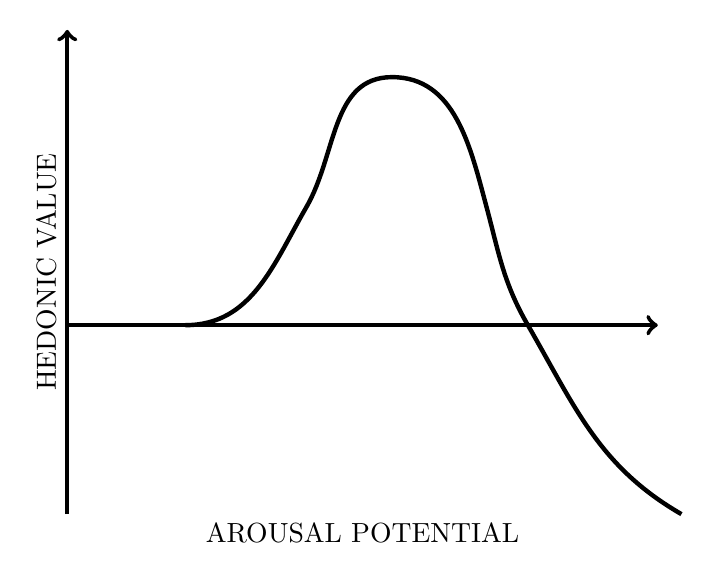
\begin{tikzpicture}[scale=0.75]
      % The image, for reference
      % \node[anchor=south west,inner sep=0] at (0,0) {\includegraphics[width=\textwidth]{wundt.png}};

      % Axes
      \draw[black,ultra thick,->] (1,0.8) -- (1,  9)   node[midway, above, sloped] {HEDONIC VALUE};     % y axis
      \draw[black,ultra thick,->] (1,4)   -- (11, 4);                                                   % x axis
      \path                       (1,0.8) -- (11, 0.8) node[midway, below]         {AROUSAL POTENTIAL}; % x axis label

      % Curve. The numbers come from tracing over wundt.png
      \draw[black,ultra thick] (3, 4)
           to[out=0,   in=240] (5.05, 6)
           to[out=60,  in=180] (6.5,  8.2)
           to[out=0,   in=105] (8.1,  6)
           to[out=-75, in=120] (8.8,  4)
           to[out=-60, in=150] (11.4, 0.8);

      % This version is closer, but a little jagged
      \iffalse
      \draw[black,ultra thick] (3, 4)
           to[out=0,   in=240] (5.05, 6)
           to[out=60,  in=225] (6,    8)
           to[out=45,  in=180] (6.5,  8.2)
           to[out=0,   in=135] (7.2,  8)
           to[out=-45, in=105] (8.1,  6)
           to[out=-75, in=120] (8.8,  4)
           to[out=-60, in=150] (11.4, 0.8);
      \fi
  \end{tikzpicture}

  \caption{The Wundt curve, reproduced from \citep{berlyne1970novelty}. The axes ``hedonic value'' and ``arousal potential'' are described as covering \textquote{reward value\dots preference or pleasure}, and \textquote{all the stimulus properties that tend to raise arousal, including novelty and complexity}, respectively.}

  \label{wundt}
\end{figure}

\emph{Artificial curiosity} (AC) describes active learning systems which are rewarded based on how interesting the input or data they discover is \citep{schmidhuber2006developmental}. Although framed in the context of \emph{reinforcement learning}, this is clearly relevant to our theory exploration setting.

As an unsupervised learning task, AC has no access to labels or meanings associated with its input; the only features it can learn are the structure and relationships inherent in the data, which is very much what we would like a theory exploration system to do. The unifying principle of AC methods is to force systems away from inputs which are not amenable to learning; either because they are so familiar that there is nothing left to learn, or so unfamiliar that they are unintelligible. The resulting behaviour is characterised by the \emph{Wundt curve} (shown in figure \ref{wundt}) \footnote{In practice, many measures avoid negative values for simplicity, in which cases we replace all negative points on the curve with zero.}, which has been used in psychology to explain human aesthetics and preferences \citep{berlyne1970novelty}.

We can divide AC approaches into two groups: the first, which we call \emph{explicit}, send inputs which follow a Wundt curve to their learning algorithm; the second, the \emph{implicit} approaches, instead modify the \emph{output} of their learning algorithm(s), such that the overall system follows a Wundt curve as an emergent property.

In the explicit case, the \emph{implicit reward} signals being learned are analogous to our notion of interestingness. A framework encompassing many examples is given in \citep{oudeyer2007intrinsic} in the context of reinforcement learning.

One particularly general measure is \emph{compression progress}: given a compressed representation of our previous observations, the ``progress'' is the space saved if we include the current observation. Observations which are incompressible or trivially compressible don't save any space, whilst observations which provide new information relevant to past experience can provide a saving. This can be translated to a theorem proving context very naturally: our observations are theorems and their proofs, whilst new theorems which generalise known results will allow us to compress their proofs.

% TODO: Examples
\citep{Schmidhuber1999}

Two sources of intrinsic reward are proposed in \citep{Hester.Stone:2012} for \emph{random forests}. A random forest is a population of decision trees, where each tree is trained on a sub-set of the available examples, each decision is made using a sub-set of the available features, and the predictions of every tree are averaged to obtain that of the forest \citep{randomforests}. The first intrinsic reward is the \emph{disagreement} between predictions; for a forest with $m$ models (trees), predicting features $x_1$ \dots $x_n$ of the state resulting from taking action $a$ in state $s$, we simply sum the Kullback-Leibler divergence $D_{\rm KL}$ of each prediction $P_1$ \dots $P_m$ from every other prediction:

\begin{equation}
  D(s,a) = \sum_{i = 1}^n \sum_{j = 1}^m \sum_{k = 1}^m D_{KL}(P_j(x_i|s,a) || P_k(x_i|s,a))
\end{equation}

$D(s,a)$ is an explicit AC reward, as it follows a Wundt curve as the complexity of transitions increases. For parts of the state space which have been fully learned, the models will agree on accurate predictions. For parts which are unlearnable, the models cannot infer any structure, and will converge to reporting the average of past observations; these predictions may not be accurate, but they will be in agreement. Hence it is the states which are amenable to learning which produce the largest disagreement.

The second intrinsic reward is simply a measure of distance from previous observations, which pushes the system towards unseen states regardless of how learnable they are (similar to the $R_{max}$ technique). This is too simple to meet our definition of AC, but it does force the models to generalise their predictions to unexplored states, acting to increase disagreement in the forest.

A key advantage of random forests is that their models are \emph{inspectable}: they not only give predictions, but also \emph{reasons} for those predictions (i.e. we can see which paths are taken through each decision tree). % TODO: The accuracy of these random forest models are compared

% TODO
\citep{Kaplan2006}
\citep{Lipson2007}
\citep{Luciw2011}
\citep{Macedo2000}
\citep{Ramik.Sabourin.Madani:2013}
\citep{Roa.Kruijff.Jacobsson:2009}
\citep{Schaul.Sun.Wierstra.ea:2011}
\citep{Schmidhuber1999}
\citep{Schmidhuber:1991}
\citep{Scott1989}
\citep{Steunebrink.Koutnik.Thorisson.ea:2013}
\citep{maher2008achieving}
\citep{meyer1991possibility}
\citep{oudeyer2004intelligent}
\citep{oudeyer2014evolution}
\citep{schmidhuber2006developmental}

% TODO: Coevolution

Whilst clearly of relevance to theory exploration, artificial curiosity is usually framed in the context of a \emph{reinforcement learning} and \emph{intrinsic reward}, especially in the field of developmental robotics. This requires non-trivial choices to be made in deciding which of its concepts are of relevance to our domain, and how they may be translated across. For example, much of developmental robotics studies continuous, real-valued sensorimotor signals which may not have any direct analogue in the manipulation of logical formulae. However, if we take a higher-level view, the study of such signals may provide insight for predicting and tuning the behaviour of off-the-shelf ATP algorithms.

The most obvious contrast between developmental robotics and theory exploration is that the latter is not physically embodied (e.g. in a robot). Embodiment has been proposed as a necessary property of intelligent systems, as it provides \emph{grounding} \citep{anderson2003embodied}. Embodiment emerged as a response to the symbolic techniques of GOFAI, and in this sense the fields of theory exploration and developmental robotics seem incompatible. Nevertheless, TE can be seen to avoid the problems of GOFAI in two ways:

\begin{itemize}

  \item Firstly, the abstract, mathematical domain being explored is not a \emph{model} of some external, physical environment; the domain \emph{is} our environment; hence there is no issue of grounding terms with some external meaning.

  \item Secondly, there is a physical aspect of TE in that \emph{resource usage} is a critical factor. If it weren't, then brute force enumeration of proofs would be a viable solution. In this sense, we can provide physical inputs to our algorithms, such as measures of time and space used.

\end{itemize}

\iffalse

\subsubsection{Universal Drives}

PhysRevLett.110.168702.pdf
Omohundro? Too physical.
\emph{Universal drives} are those

\fi

\subsection{Statistics of Formal Systems}

The core problem of assigning ``interestingness'' to logical formulae is the application of statistical reasoning to the discrete, semantically-rich domain of formal systems. This problem has been tackled from various directions for a variety of reasons; here we summarise those contributions which seem of particular importance for theory exploration.

\subsubsection{Relevance Filtering}
\label{relevance}

% TODO
\citep{kuhlwein2012overview}

The combinatorial nature of formal systems causes many proof search methods, such as resolution, to have exponential complexity \citep{haken1985intractability}; hence even a modest size increase can turn a trivial problem into an intractable one. Finding efficient alternatives for such algorithms, especially those which are NP-complete (e.g. determining satisfiability) or co-NP-complete (e.g. determining tautologies), seems unlikely, as it would imply progress on the famously intractable open problems of $\text{P} = \text{NP}$ and $\text{NP} = \text{co-NP}$. On the other hand, we can turn this difficulty around: a modest \emph{decrease} in size may turn an intractable problem into a solvable one. We can ensure that the solutions to these reduced problems coincide with the original if we only remove \emph{redundant} information. This leads to the idea of \emph{relevance filtering}.

Relevance filtering simplifies a proof search problem by removing from consideration those clauses (axioms, definitions, lemmas, etc.) which are deemed \emph{irrelevant}. The technique is used in Sledgehammer during its translation of Isabelle/HOL theories to statements in first order logic: rather than translating the entire theory, only a sub-set of relevant clauses are included. This reduces the size of the problem and speeds up the proof search, but it creates the new problem of determining when a clause is relevant: how do we know what will be required, before we have the proof?

The initial approach, known as \textsc{MePO} (from \emph{Meng-Paulson} \citep{meng2009lightweight}), gives each clause a score based on the proportion $m / n$ of its symbols which are ``relevant'' (where $n$ is the number of symbols in the clause and $m$ is the number which are relevant). Initially, the relevant symbols are those which occur in the goal, but whenever a clause is found which scores more than a particular threshold, all of its symbols are then also considered relevant. There are other heuristics applied too, such as increasing the score of user-provided facts (e.g. given by keywords like \texttt{using}), locally-scoped facts, first-order facts and rarely-occuring facts. To choose $r$ relevant clauses for an ATP invocation, we simply order the clauses by decreasing score and take the first $r$ of them.

Recently, a variety of alternative algorithms have also been investigated, including:

\begin{description}

  \item{\textsc{MaSH}}: Machine Learning for SledgeHammer \citep{kuhlwein2013mash}. The distinguishing feature of \textsc{MaSH} is its use of ``visibility'', which is essentially a dependency graph of which theorems were used in the proofs of which other theorems; although theorems are represented as abstract sets of features. To select relevant clauses for a goal, the set of clauses which are visible from the goal's components is generated; this is further reduced by (an efficient approximation of) a naive Bayes algorithm.

  \item{\textsc{MOR}}: \emph{Multi-output ranking} uses a support vector machine (SVM) approach for selecting relevant axioms from the Mizar Mathematical Library for use by the Vampire ATP system \citep{alama2014premise}. \iffalse TODO: describe the kernel, as that's the interesting bit \fi It compares favourably to \textsc{SNoW} and \textsc{SInE}.

  % TODO:
  \item{\textsc{SInE}}
  \item{\textsc{BliStr}}
  \item{\textsc{HOLyHammer}}
  \item{\textsc{MoMM}}
  \item{\textsc{SNoW}}
  \item{\textsc{MPTP 0.2}}
  \item{\textsc{MaLARea}}
  \item{\textsc{MaLARea SG1}}

\end{description}

\subsubsection{Clustering}
\label{clustering}

% TODO: ML4PG
\citep{journals/corr/abs-1212-3618}
% TODO: ACL2(ml) (also examples section)
\citep{heras2013proof}

\subsubsection{Probability of Sentences}

The most important property of a logical formula is its truth value. Although we may be able to determine some truth values exactly, e.g. using decision or semi-decision procedures, it may be more efficient to \emph{approximate} truth values. One straightforward extension of truth values is \emph{probabilities}, where we can assign probability $1$ to formulae which are known to be true, $0$ to formulae known to be false, and intermediate values to those which we do not yet know.

% TODO
\citep{Hutter.Lloyd.Ng.ea:2013}

\subsubsection{Interestingness in Concept Formation}
\label{conceptformation}

% TODO:
\citep{Montano-Rivas.McCasland.Dixon.ea:2012}
\citep{Piantadosi.Tenenbaum.Goodman:2012}
\citep{Wille:2005}
\citep{colton1999automatic}
\citep{colton2000agent}
\citep{colton2012automated}
\citep{lenat1977automated}
\citep{mullerunderstanding}
\citep{Bundy.Cavallo.Dixon.ea:2015}
\citep{johansson2009isacosy}
\citep{spector2008genetic}
\citep{colton2012automated}
 \citep{geng2006interestingness}
% TODO: How does https en.wikipedia.org/wiki/Discovery system relate?

% However, this search space grows exponentially in the length of the proofs, which is unfortunate since proof length has been proposed as an approximate measure of how interesting a theorem is \cite[\S~10.2.1]{colton2012automated}.

% Alan Bundy et al

% Eurisko, AM, etc.?

\subsubsection{Learning From Structured Data}

One major difficulty with formal mathematics as a domain in which to apply statistical machine learning is the use of \emph{structure} to encode information in objects. In particular, \emph{trees} appear in many places: from inductive datatypes, to recursive function definitions; from theorem statements, to proof objects. Such nested structures may extend to arbitrary depth, which makes them difficult to represent with a fixed number of features, as is expected by most machine learning algorithms. Here we review a selection of solutions to this problem, and compare their distinguishing properties.

\paragraph{Feature Extraction}\label{featureextraction}

\emph{Feature extraction} is a common pre-processing step for machine learning (ML). Rather than feeding ``raw'' data straight into our ML algorithm, we only learn a sample of \emph{relevant} details, known as \emph{features}. This has two benefits:

\begin{itemize}
  \item \emph{Feature vectors} (ordered sets of features) are chosen to be more compact than the data they're extracted from: feature extraction is \emph{lossy compression}. This reduces the size of the ML problem, improving efficiency (e.g. running time).
  \item We avoid learning irrelevant details such as the encoding system used, improving \emph{data} efficiency (the number of samples required to spot a pattern).
\end{itemize}

Another benefit of feature extraction is to \emph{normalise} the input data to a fixed-size representation. Many ML algorithms only work with fixed-size inputs; for example, the popular \emph{backpropagation} \citep{Russell:2003:AIM:773294} algorithm works on models with \emph{fixed} topology (e.g. \emph{artificial neural networks} with fixed connections between nodes). This requires some form of pre-processing in domains where the size of each input is not known, may vary or may even be unbounded.

For example, in the case of \emph{online} learning we must make predictions/decisions before seeing all of the inputs. Unbounded input appears in domains such as programming and theorem proving, where individual term may be trees of unbounded depth. In these situations we need a mapping from arbitrary inputs to a fixed representation which is amenable to learning.

As an example, say we want to learn relationships between the following program fragments:

\begin{lstlisting}[language=Haskell, xleftmargin=.2\textwidth, xrightmargin=.2\textwidth]
data Maybe a = Nothing | Just a

data Either a b = Left a | Right b
\end{lstlisting}

We might hope our algorithm discovers relationships like:

\begin{itemize}
  \item Both are valid Haskell code.
  \item Both describe datatypes.
  \item Both datatypes have two constructors.
  \item \hs{Either} is a generalisation of \hs{Maybe} (we can define \hs{Maybe a = Either () a} and \hs{Nothing = Left ()}).
  \item There is a symmetry in \hs{Either}: \hs{Either a b} is equivalent to \hs{Either b a} if we swap occurences of \hs{Left} and \hs{Right}.
  \item It is trivial to satisfy \hs{Maybe} (using \hs{Nothing}).
  \item It is not trivial to satisfy \hs{Either}; we require an \hs{a} or a \hs{b}.
\end{itemize}

However, this is too optimistic. Without our domain-knowledge of Haskell, an ML algorithm cannot impose any structure on these fragments, and will treat them as strings of bits. Our high-level hopes are obscured by low-level details: the desirable patterns of Haskell types are mixed with undesirable patterns of ASCII bytes, of letter frequency in English words, and so on.

In theory we could throw more computing resources and data at a problem, but available hardware and corpora are always limited. Instead, feature extraction lets us narrow the ML problem to what we, with our domain knowlege, consider important.

There is no \emph{fundamental} difference between raw representations and features: the identity function is a valid feature extractor. Likewise, there is no crisp distinction between feature extraction and machine learning: a sufficiently-powerful learner doesn't require feature extraction, and a sufficiently-powerful feature extractor doesn't require any learning! \footnote{Consider a classification problem, to assign a label $l \in L$ to each input. If we only extract a single feature $f \in L$, we have solved the classification problem without using a separate learning step.}

Rather, the terms are distinguished for purely \emph{practical} reasons: by separating feature extraction from learning, we can distinguish straightforward, fast data transformation (feature extraction) from complex, slow statistical analysis (learning). This allows for modularity, separation of concerns, and in particular allows ``off-the-shelf'' ML to be re-used across a variety of different domains.

Even if we have no domain knowledge, we can still use a feature extraction phase to improve efficiency: first we learn a compact representation for our data, for example using \emph{autoencoding}; then we use that encoder as a feature extractor for our main learning task. This stacking of one learning algorithm on top of another, especially with greedy learning of each layer, has lead to the recent trend of \emph{deep learning}.

\paragraph{Truncation and Padding}

The simplest way to limit the size of our inputs is to truncate anything larger than a particular size (and pad anything smaller). This is the approach taken by ML4PG \citep{journals/corr/abs-1302-6421}, which limits itself to trees with at most 10 levels and 10 elements per level; each tree is converted to a $30 \times 10$ matrix (3 values per tree node) and learning takes place on these normalised representations.

Truncation is unsatisfactory in the way it balances \emph{data} efficiency with \emph{time} efficiency. Specifically, truncation works best when the input data contains no redundancy and is arranged with the most significant data first (in a sense, it is ``big-endian''). The less these assumptions hold, the less we can truncate. Since many ML algorithms scale poorly with input size, we would prefer to eliminate the redundancy using a more aggressive algorithm, to keep the resulting feature size as low as possible.

\paragraph{Dimension Reduction}

A more sophisticated approach to the problem of reducing input size is to view it as a \emph{dimension reduction} technique: our inputs can be modelled as points in high-dimensional spaces, which we want to project into a lower-dimensional space ($\left\{ {0, 1} \right\}^N$ in the case of $N$-bit vectors).

Truncation is a trivial dimension reduction technique: take the first $N$ coordinates (bits). More sophisticated projection functions consider the \emph{distribution} of the points, and project with the hyperplane which preserves as much of the variance as possible (or, equivalently, reduces the \emph{mutual information} between the points).

There are many techniques to find these hyperplanes, such as \emph{principle component analysis} (PCA) and \emph{autoencoding}; however, since these techniques are effectively ML algorithms in their own right, they suffer some of the same constraints we're trying to avoid:

\begin{itemize}
  \item They operate \emph{offline}, requiring all input points up-front
  \item All input points must have the same dimensionality
\end{itemize}

In particular, the second constraint is precisely what we're trying to avoid. Sophisticated dimension reduction is still useful for \emph{compressing} large, redundant features into smaller, information-dense representations, and as such provides a good complement to truncation.

The requirement for offline ``batch'' processing is more difficult to overcome, since any learning we perform for feature extraction will interfere with the core learning algorithm that's consuming these features (this is why deep learning is often done greedily).

\paragraph{Sequencing}

The task of dimension reduction changes when we consider \emph{structured} data. Recursive structures, like trees and lists, have \emph{fractal} dimension: adding layers to a recursive structure gives us more \emph{fine-grained} features, rather than \emph{orthogonal} features. For data mining context-free languages (e.g. those of programming and theorem-proving systems), we will mainly be concerned with tree structures of variable size.

Any investigation of variable-size input would be incomplete without mentioning \emph{sequencing}. This is a lossless approach, which splits the input into fixed-size \emph{chunks}, which are fed into an appropriate ML algorithm one at a time. The sequence is terminated by a sentinel; an ``end-of-sequence'' marker which, by construction, is distinguishable from the data chunks. This technique allows us to trade \emph{space} (the size of our input) for \emph{time} (the number of chunks in a sequence).

Not all ML algorithms can be adapted to accept sequences. One notable approach is to use \emph{recurrent ANNs} (RANNs), which allow arbitrary connections between nodes, including cycles. Compared to \emph{feed-forward} ANNs (FFANNs), which are acyclic, the \emph{future output} of a RANN may depend arbitrarily on its \emph{past inputs} (in fact, RANNs are universal computers).

The main problem with RANNs, compared to the more widely-used FFANNs, is the difficulty of training them. If we extend the standard backpropagation algorithm to handle cycles, we get the \emph{backpropagation through time} algorithm \citep{werbos1990backpropagation}. However, this suffers a problem known as the \emph{vanishing gradient}: error values decay exponentially as they propagate back through the cycles, which prevents effective learning of delayed dependencies, undermining the main advantage of RANNs. The vanishing gradient problem is the subject of current research, with countermeasures including \emph{neuroevolution} (using evolutionary computation techniques to train an ANN) and \emph{long short-term memory} (LSTM; introducing a few special, untrainable nodes to persist values for long time periods \citep{hochreiter1997long}).

The application of \emph{kernel methods} to structured information is discussed in \citep{Gartner2003}, where the input data (including sequences, trees and graphs) are represented using \emph{generative models}, such as hidden Markov models, of a fixed size.

% TODO
\citep{Gartner2003}
\citep{Oveisi.Oveisi.Erfanian.ea:2012}
\citep{bakir2007predicting}
\citep{conf/ijcai/Plate91}
\citep{goller1996learning}
\citep{kwasny1995tail}
\citep{pollack1990recursive}
\citep{zanzotto2012distributed}

\iffalse

Machine learning over structured data:
1D is common: parsing natural language
2D is common; images
Trees are fractal
Backpropagation through structure
LSTM with recursive structure
Most work tries to identify structure; we already have it

Recurrent neural networks
Backpropagation through structure

\fi

\section{Future Work}
\label{future}

\iffalse
TODO

interestingness
\fi

\iffalse

QuickSpec: extend or extinguish?

Improve and find other use cases/scenarios for clustering and feature extraction

Other directions for Theory Exploration?

How about systems based on term rewriting, logic programming, etc.?
\fi

\section{Conclusion}
\label{conclusion}

\bibliographystyle{plain}
\bibliography{../Bibtex}

\end{document}
